%! Mode:: "TeX:UTF-8"
%! TEX program = xelatex
\PassOptionsToPackage{quiet}{xeCJK}
\documentclass[withoutpreface,bwprint]{cumcmthesis}
\usepackage{etoolbox}
\BeforeBeginEnvironment{tabular}{\zihao{-5}}
\usepackage[numbers,sort&compress]{natbib}  % 文献管理宏包
\usepackage[framemethod=TikZ]{mdframed}  % 框架宏包
\usepackage{url}  % 网页链接宏包
\usepackage{subcaption}  % 子图宏包
\usepackage{float}  % 浮动体宏包

\newcolumntype{C}{>{\centering\arraybackslash}X}
\newcolumntype{R}{>{\raggedleft\arraybackslash}X}
\newcolumntype{L}{>{\raggedright\arraybackslash}X}

\title{全国大学生数学建模竞赛论文模板}  % 论文标题
\tihao{}  % 题号
\baominghao{}  % 报名号
\schoolname{}  % 学校
\membera{}  % 队员a
\memberb{}  % 队员b
\memberc{}  % 队员c
\supervisor{}  % 指导老师
\yearinput{}
\monthinput{}
\dayinput{}

%%%%%%%%%%%%%%%%%%%%%%%%%%%%%%%%%%%%%%%%%%%%%%%%%%%%%%%%%%%%%
%% 正文
\begin{document}

\maketitle
\begin{abstract}
摘要

\textbf{对于问题一,}

\textbf{对于问题二,}

\textbf{对于问题三,}

\textbf{对于问题四,}

最后,



\keywords{关键词\quad  关键词\quad  关键词\quad  关键词 \quad 关键词}
\end{abstract}
%%%%%%%%%%%%%%%%%%%%%%%%%%%%%%%%%%%%%%%%%%%%%%%%%%%%%%%%%%%%% 

% \tableofcontents  % 目录
% \newpage

%%%%%%%%%%%%%%%%%%%%%%%%%%%%%%%%%%%%%%%%%%%%%%%%%%%%%%%%%%%%%  
\section{问题重述}
\subsection{问题背景}
丝绸之路作为古代中西方文化交流的核心通道,玻璃是早期贸易往来的重要物证。
早期西亚和埃及的玻璃多以珠形饰品传入我国,我国古代吸收其技术后,
利用本土原料制作玻璃,虽外观与外来品相似,但因助熔剂差异(如铅矿石、草木灰等),
化学成分截然不同,形成了铅钡玻璃(我国自创,以楚文化为代表)、
高钾玻璃(流行于岭南及东南亚、印度等区域)等本土特色品种。
古代玻璃因埋藏环境易风化,风化过程中元素交换导致成分比例改变,
影响类别判断,而部分风化文物表面仍保留未风化区域,为成分研究提供了特殊样本,
对于研究古代中国社会和玻璃工艺具有很高的价值。

%%%%%%%%%%%%%%%%%%%%%%%%%%%%%%%%%%%%%%%%%%%%%%%%%%%%%%%%%%%%% 

\subsection{问题要求}

\textbf{问题1}  
分析玻璃文物的表面风化状态与其类型(高钾玻璃 / 铅钡玻璃)、
纹饰、颜色之间的关联;结合玻璃类型,
总结文物表面有无风化时化学成分含量的统计规律;
并基于风化点的检测数据,预测其风化前的化学成分含量。

\textbf{问题2}  
依据附件数据,提炼高钾玻璃与铅钡玻璃的分类规律;
针对这两类玻璃,分别选取合适的化学成分进行亚类划分,
明确具体的划分方法及结果,并分析该分类结果的合理性与敏感性。

\textbf{问题3} 
对附件表单 3 中未知类别的玻璃文物,通过分析其化学成分鉴别其所属类型
(高钾玻璃或铅钡玻璃),并对该分类结果的敏感性进行分析。

\textbf{问题4}  
针对高钾玻璃和铅钡玻璃这两类不同的文物样品,
分别分析其内部化学成分之间的关联关系,
并比较两类玻璃在化学成分关联关系上的差异性。
%%%%%%%%%%%%%%%%%%%%%%%%%%%%%%%%%%%%%%%%%%%%%%%%%%%%%%%%%%%%% 

\section{问题分析}
\subsection{问题一分析}
对于问题一,

\subsection{问题二分析}	
对于问题二,

\subsection{问题三分析}
对于问题三,

\subsection{问题四分析}
对于问题四,

%%%%%%%%%%%%%%%%%%%%%%%%%%%%%%%%%%%%%%%%%%%%%%%%%%%%%%%%%%%%% 

\section{模型假设}

为简化问题,本文做出以下假设:

\begin{itemize}[itemindent=2em]
\item 假设1
\item 假设2
\item 假设3
\end{itemize}

%%%%%%%%%%%%%%%%%%%%%%%%%%%%%%%%%%%%%%%%%%%%%%%%%%%%%%%%%%%%% 

\section{符号说明}
\begin{table}[H]
\centering
\begin{tabularx}{\textwidth}{CLC}
\toprule
符号    & 说明    & 单位 \\
\midrule
$m     $& 质量 & $kg$ \\
$V     $& 体积 & $m^3$ \\
\bottomrule
\end{tabularx}
\label{tab:符号说明}
\end{table}


%%%%%%%%%%%%%%%%%%%%%%%%%%%%%%%%%%%%%%%%%%%%%%%%%%%%%%%%%%%%% 

\section{问题一的模型的建立和求解}
\subsection{玻璃类型、颜色、纹饰与风化的关系}
首先我们对表单2中各文物采样点的化学成分进行累加,其中样本编号为15、17的文物
化学成分总和分别为79.47\%、71.89\%,不满足题目对成分比例累加和介于 
85\%~105\%之间的要求,因此我们将其剔除。

为了分析表面风化与玻璃类型、纹饰、颜色之间的关系,我们分别统计
(表面风化,玻璃类型)(表面风化,纹饰)(表面风化,颜色)这三个二元组
的列联表数据,并进行了可视化。

% 表1:表面风化与颜色的列联表(单独一行)
\begin{table}[htbp]
    \centering
    \caption{表面风化与颜色的列联表}
    \begin{tabular}{lcccccccc}
        \toprule
        \multirow{2}{*}{表面风化} & \multicolumn{8}{c}{颜色} \\
        \cmidrule(lr){2-9}
        & 浅绿 & 浅蓝 & 深绿 & 深蓝 & 紫 & 绿 & 蓝绿 & 黑 \\
        \midrule
        无风化 & 2 & 6 & 3 & 2 & 2 & 1 & 6 & 0 \\
        风化 & 1 & 12 & 4 & 0 & 2 & 0 & 9 & 2 \\
        \bottomrule
    \end{tabular}
\end{table}

% 表2和表3并排显示(同一行)
\begin{table}[htbp]
    \centering
    % 表2:表面风化与纹饰
    \caption{表面风化与纹饰、玻璃类型的列联表} % 总标题(可选)
    \begin{subtable}[t]{0.45\textwidth}
        \centering
        \caption{表面风化与纹饰的列联表}
        \begin{tabular}{lccc}
            \toprule
            \multirow{2}{*}{表面风化} & \multicolumn{3}{c}{纹饰} \\
            \cmidrule(lr){2-4}
            & A & B & C \\
            \midrule
            无风化 & 11 & 0 & 11 \\
            风化 & 11 & 6 & 17 \\
            \bottomrule
        \end{tabular}
    \end{subtable}
    \hspace{-15mm}% 两表之间的水平间距
    % 表3:表面风化与玻璃类型
    \begin{subtable}[t]{0.45\textwidth}
        \centering
        \caption{表面风化与玻璃类型的列联表}
        \begin{tabular}{lcc}
            \toprule
            \multirow{2}{*}{表面风化} & \multicolumn{2}{c}{类型} \\
            \cmidrule(lr){2-3}
            & 铅钡 & 高钾 \\
            \midrule
            无风化 & 12 & 10 \\
            风化 & 28 & 6 \\
            \bottomrule
        \end{tabular}
    \end{subtable}
\end{table}

\begin{figure}[H]
\centering
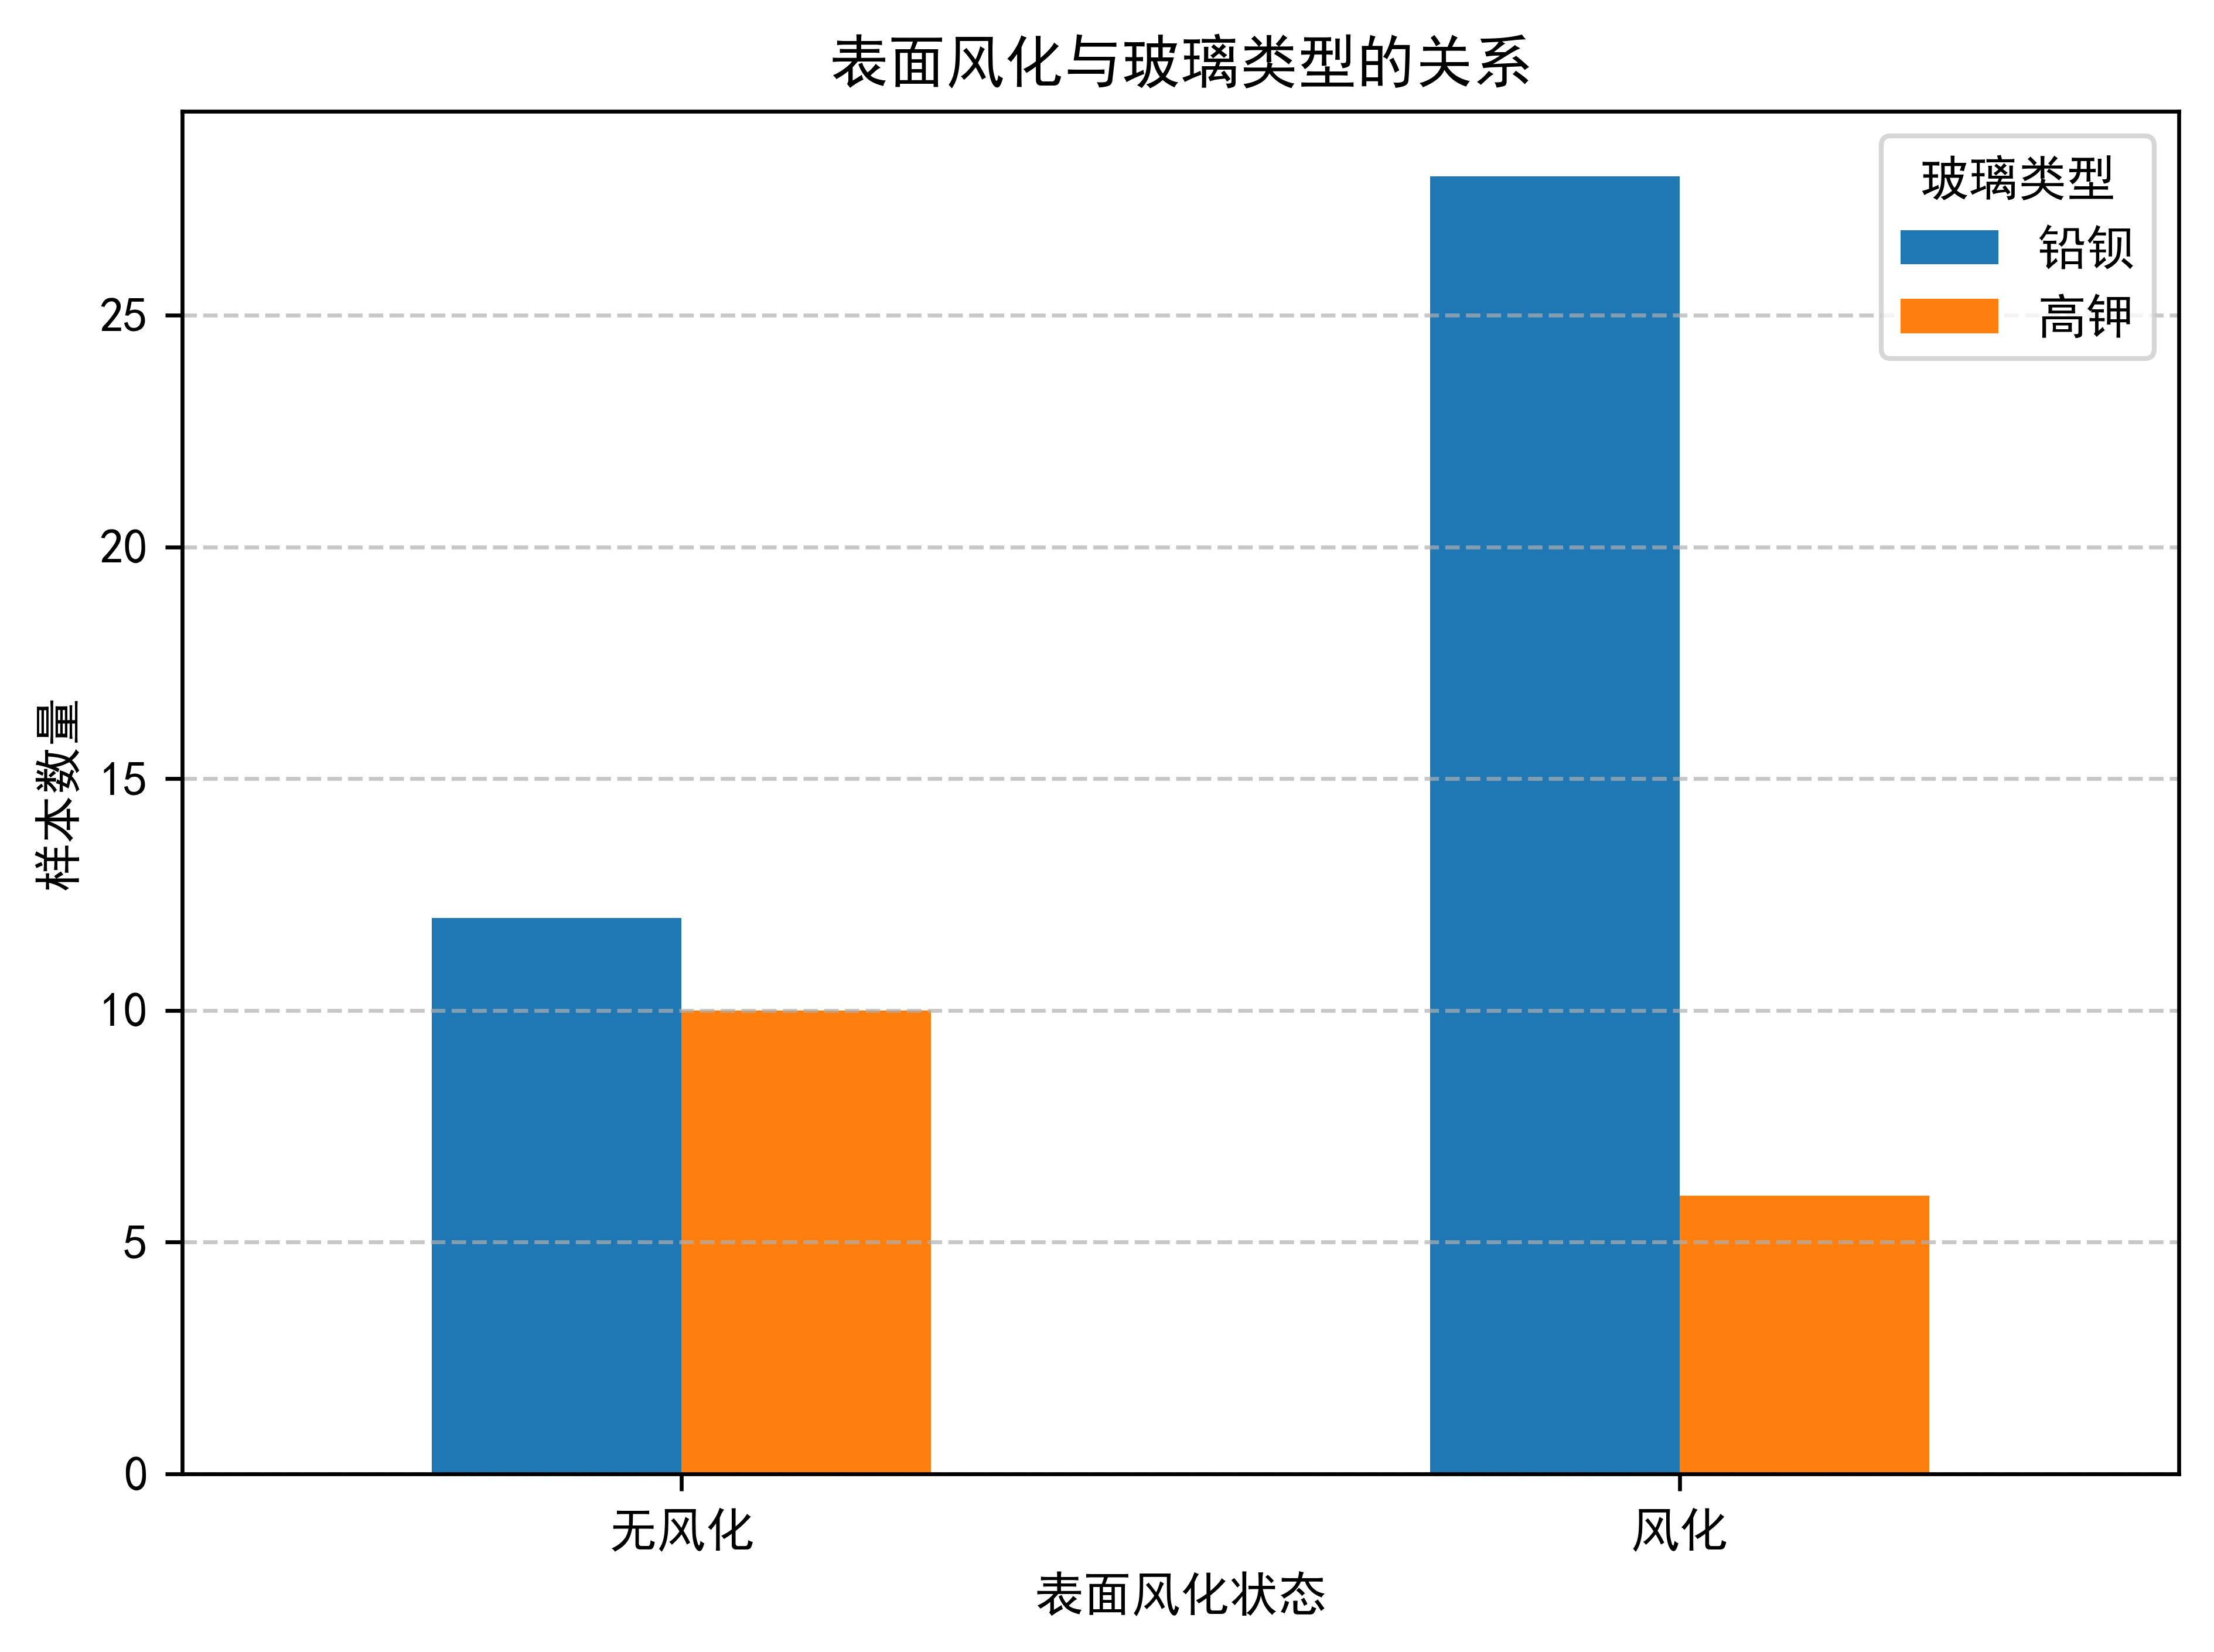
\includegraphics[width=0.6\textwidth]{figures/1.1/1-1.png}
\caption{表面风化与玻璃类型}
\label{fig:表面风化与玻璃类型}
\end{figure}

\begin{figure}[H]
\centering
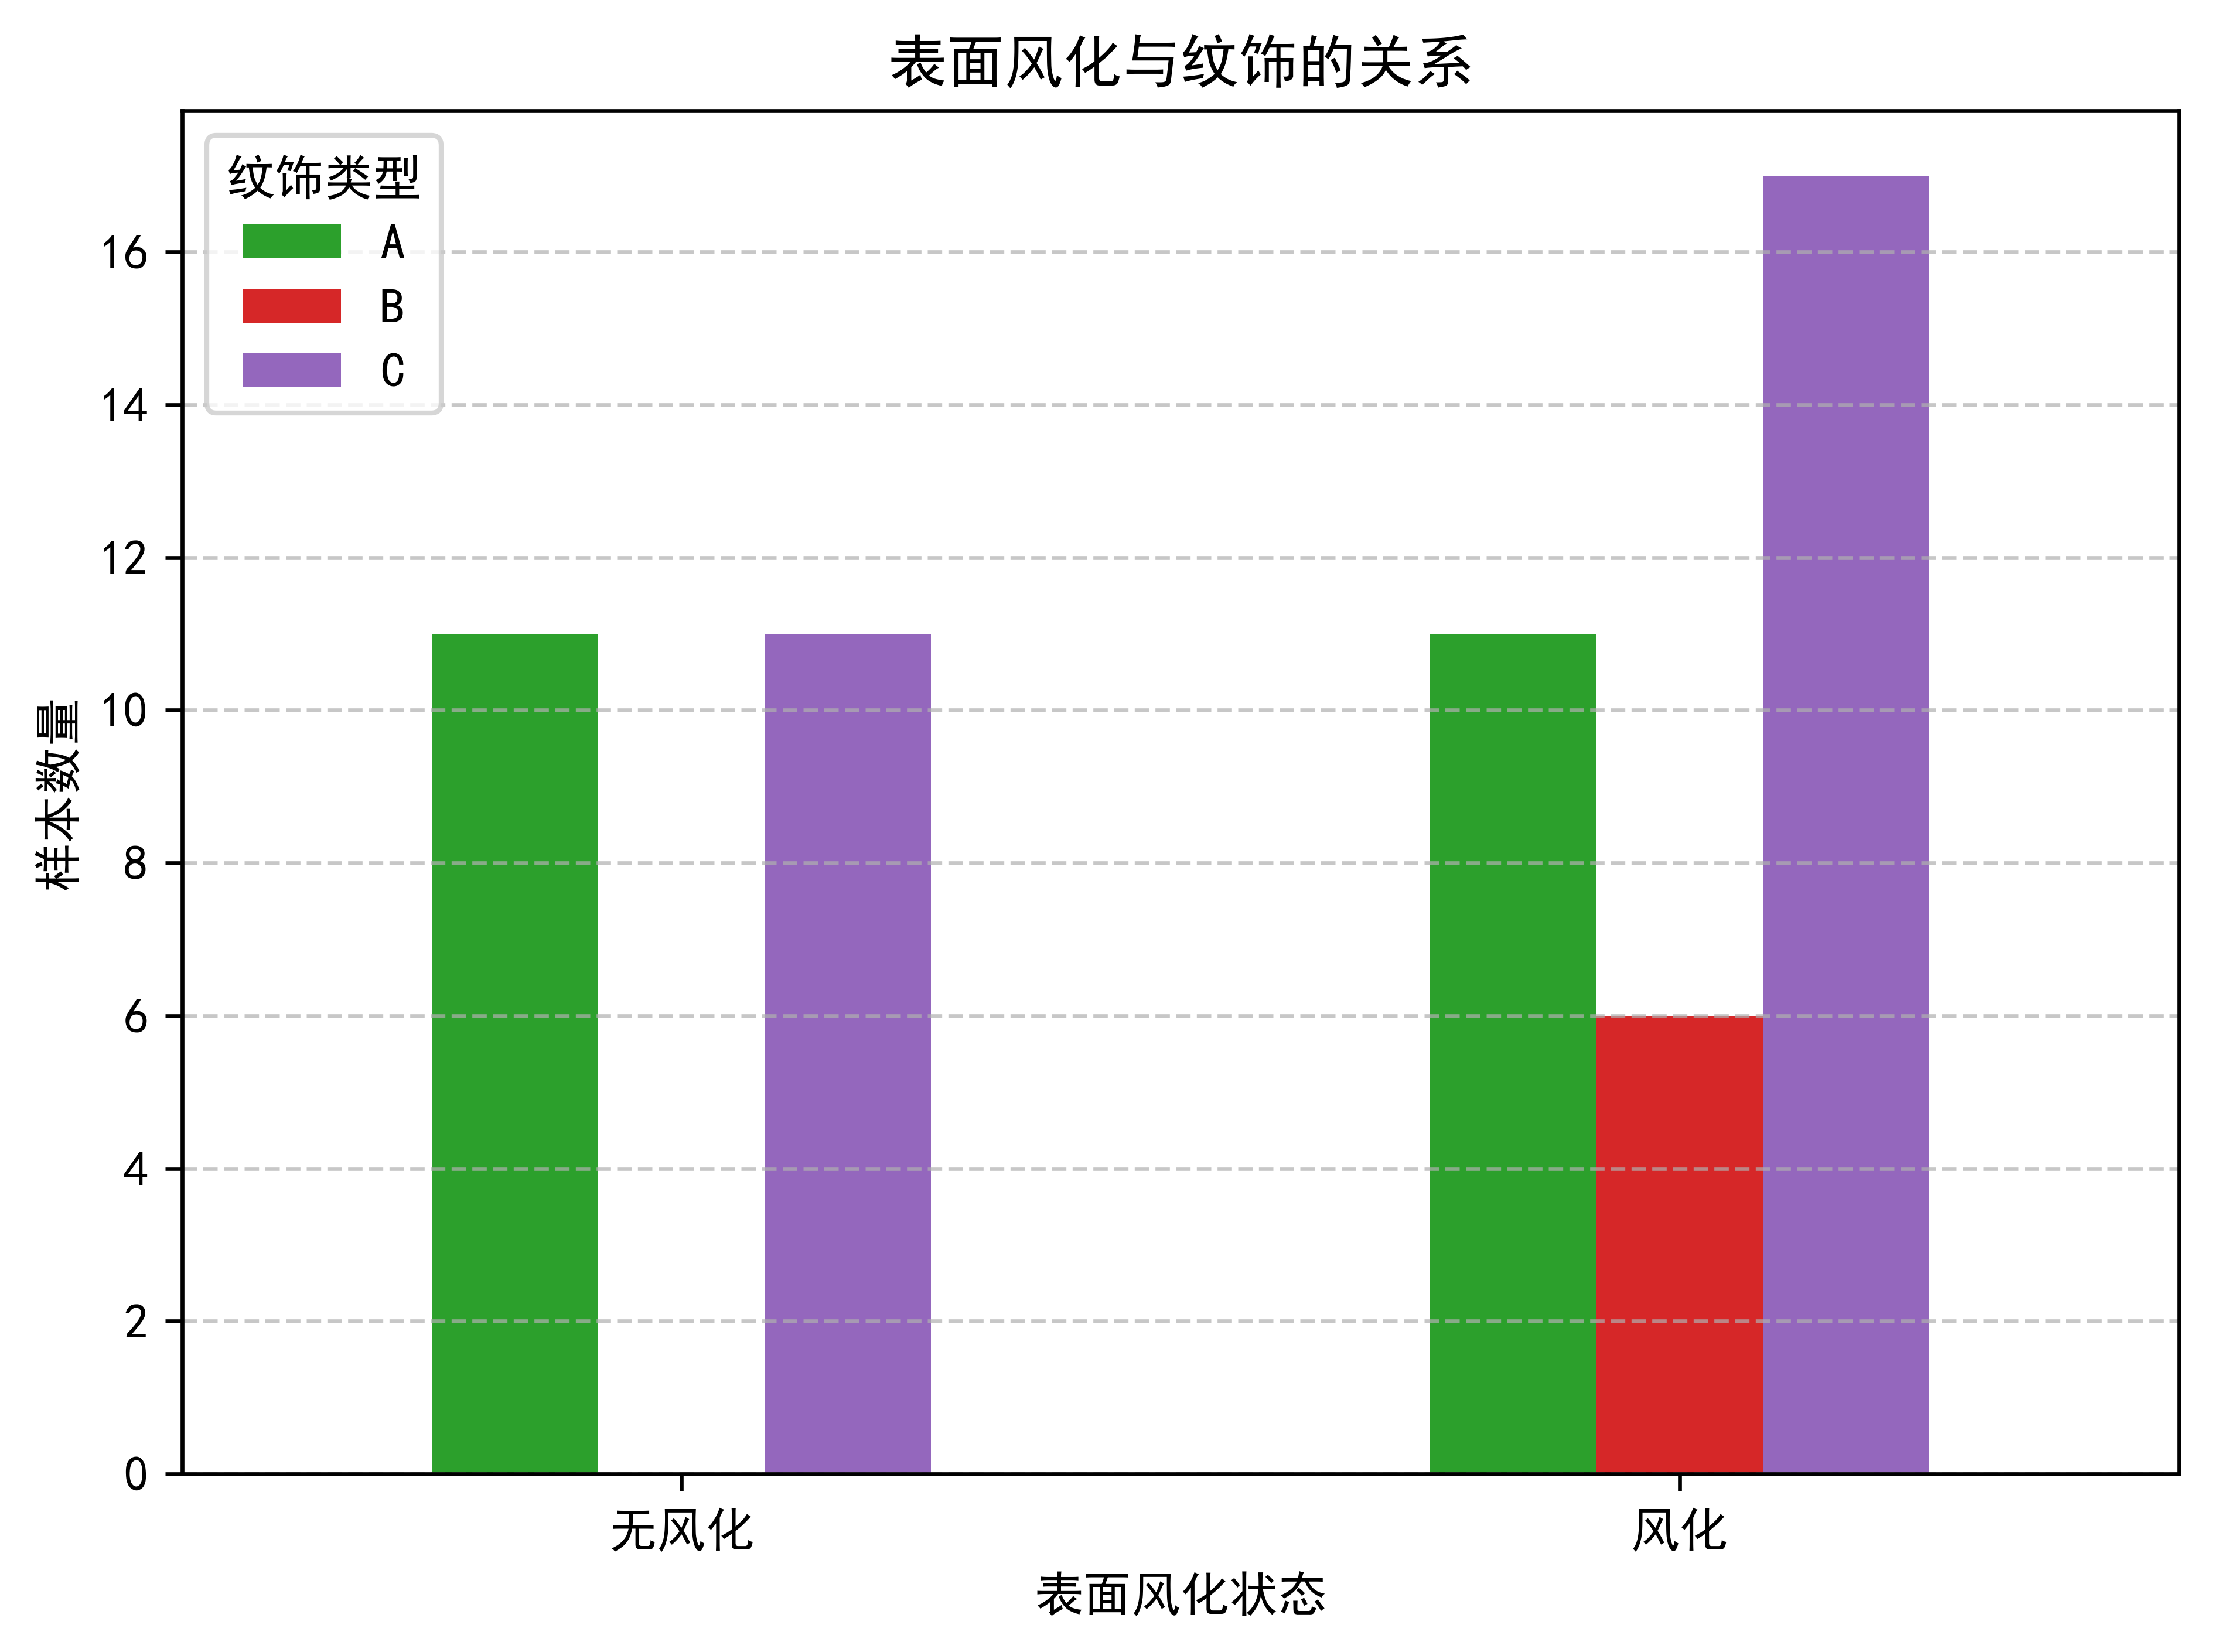
\includegraphics[width=0.6\textwidth]{figures/1.1/1-2.png}
\caption{表面风化与纹饰}
\label{fig:表面风化与纹饰}
\end{figure}

\begin{figure}[H]
\centering
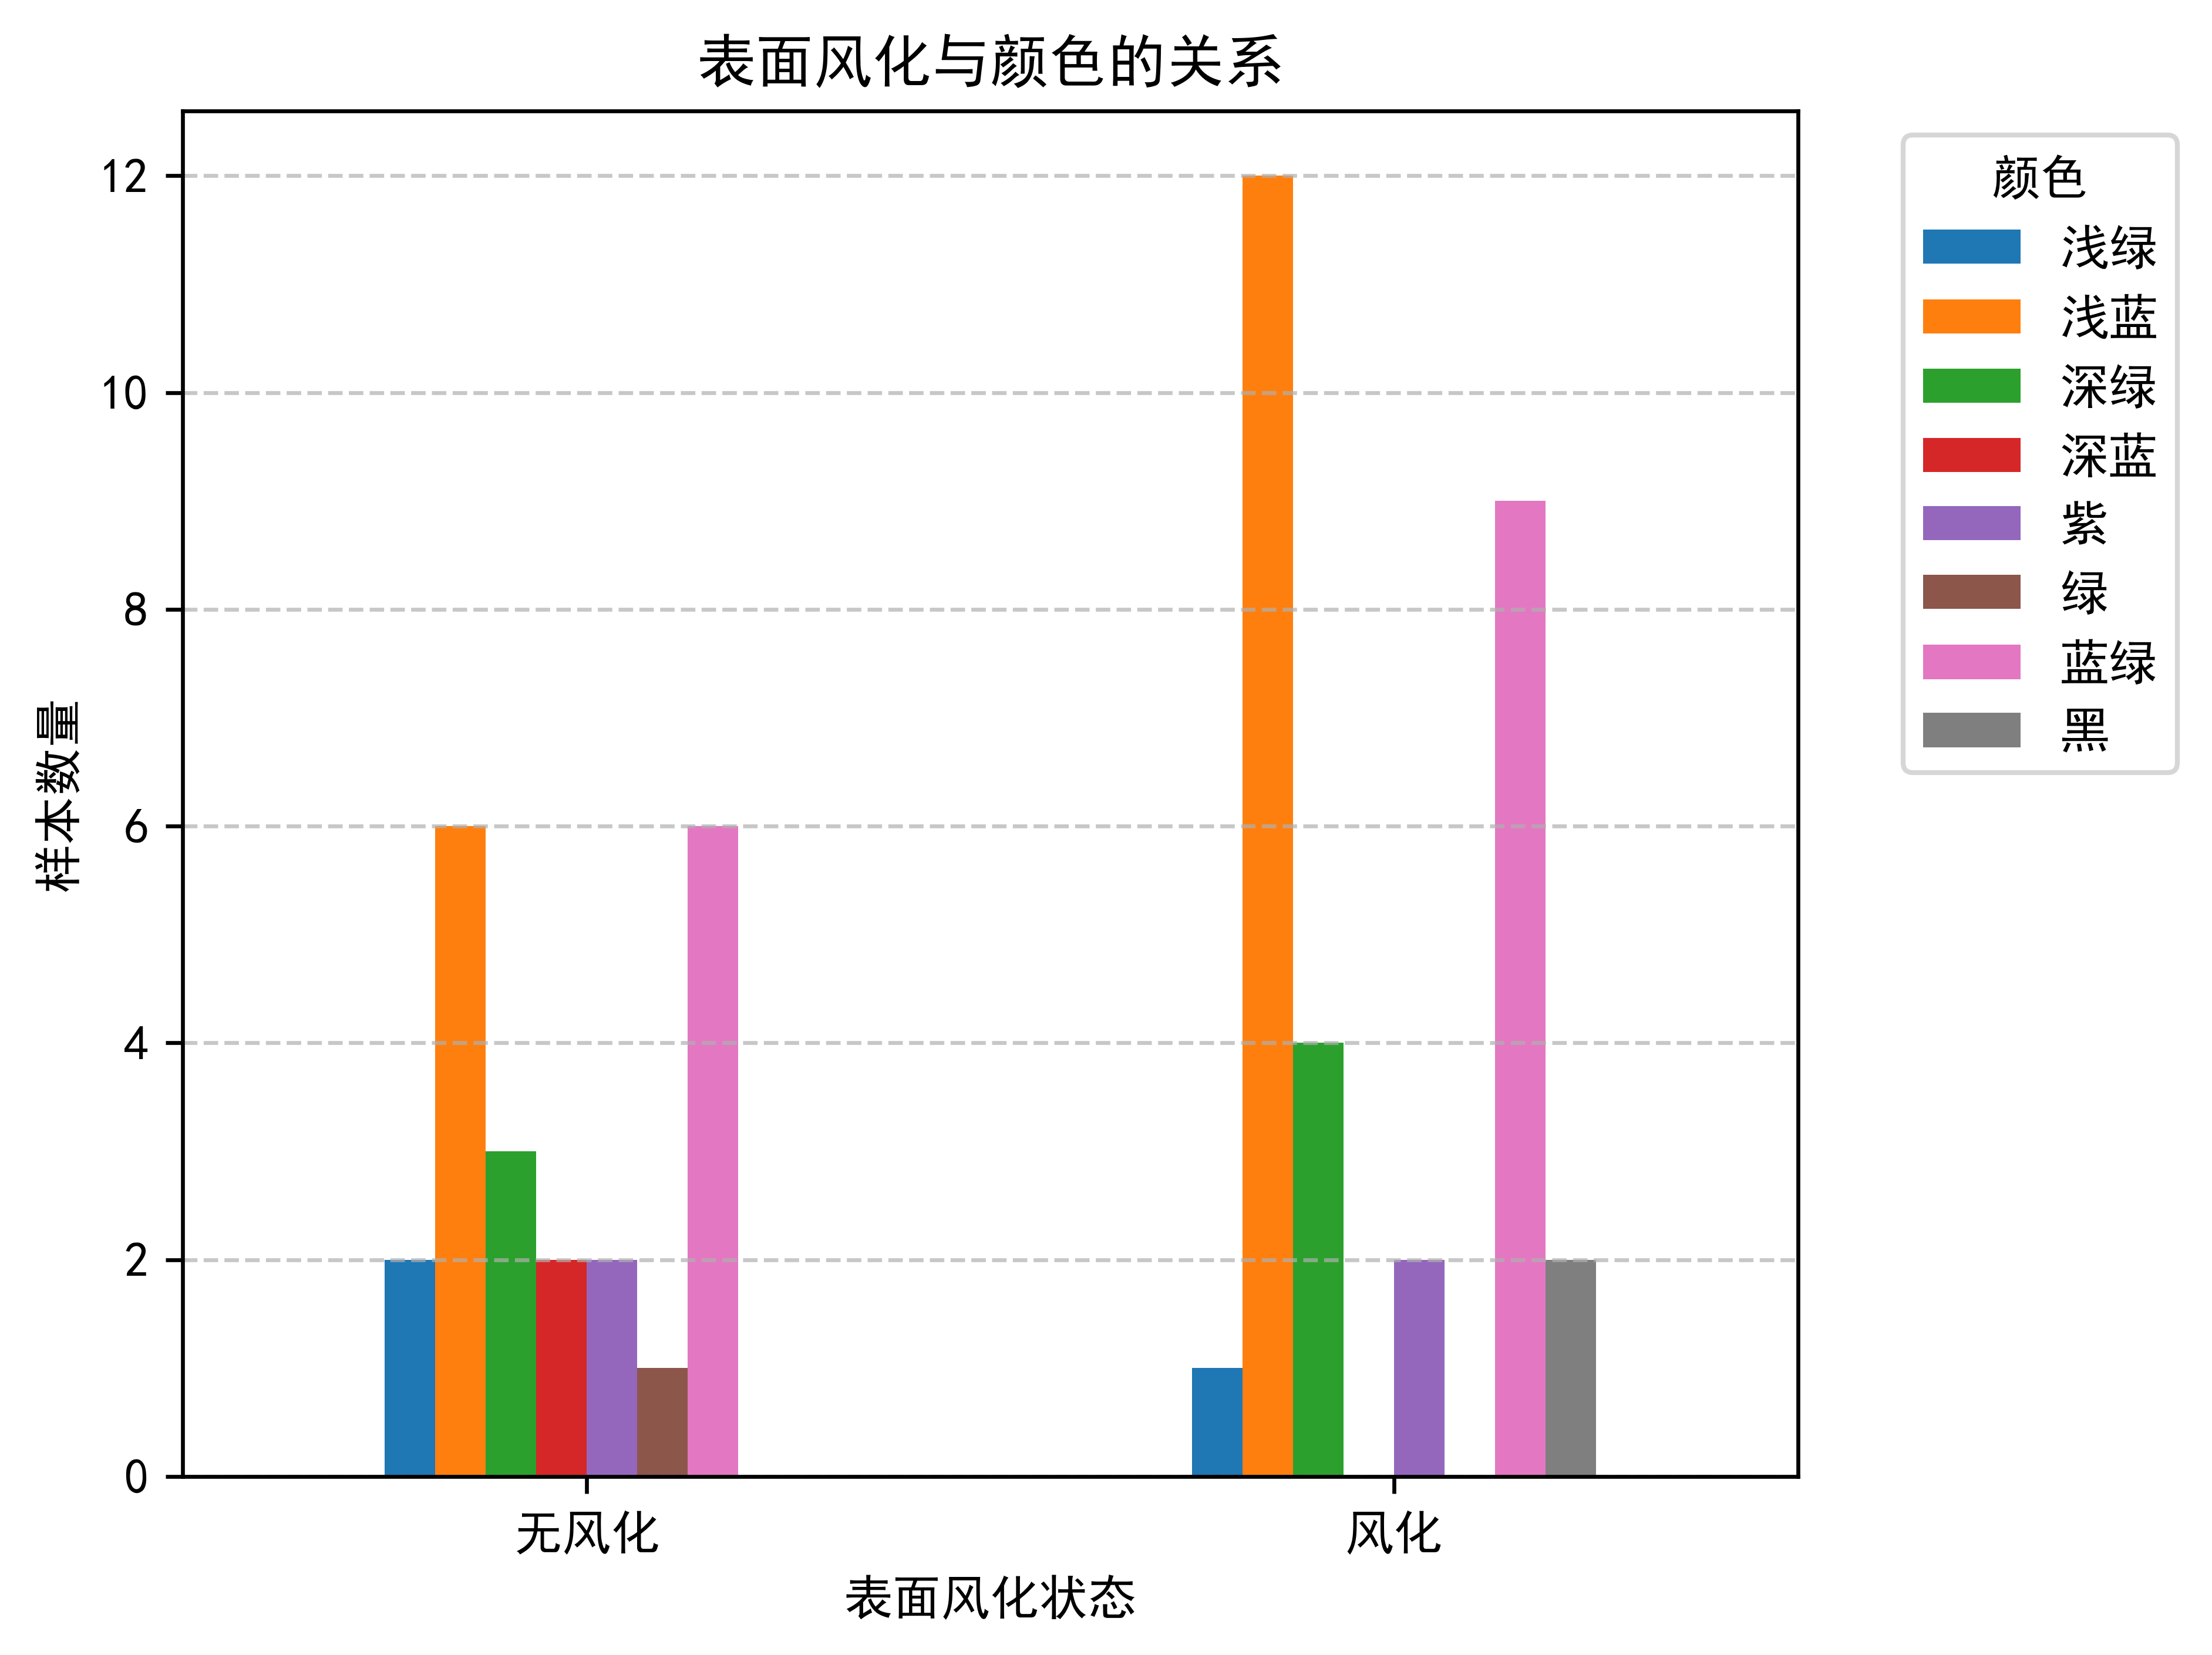
\includegraphics[width=0.6\textwidth]{figures/1.1/1-3.png}
\caption{表面风化与颜色}
\label{fig:表面风化与颜色}
\end{figure}

为了量化表面风化与玻璃类型、纹饰、颜色之间的关系,我们引入了卡方检验。
卡方检验用于检验两个分类变量是否独立,通过比较观测值与期望值的差异,
用 $\chi^2$ 统计量判断关联是否显著,适用于计数数据。

%引用公式\cref{eq:公式1}。

\begin{equation}
\label{eq:公式1}
\chi^2 = \sum \frac{(O - E)^2}{E}
\end{equation}

其中:
 $\chi^2$:卡方统计量;
 $O$:实际观测频数;
 $E$:理论期望频数;
 $\sum$:对所有单元格求和。

分别带入(表面风化,玻璃类型)(表面风化,纹饰)(表面风化,颜色)的
列联表数据可以求出$\chi^2$值和$p$值,我们这里取$p<0.005$。从下面的表格中我们可以看出,
是否风化与玻璃类型之间存在显著关系,而风化与纹饰、颜色之间则不存在显著关系。

\begin{table}[htbp]
    \centering
    \caption{卡方检验结果}
    \begin{tabular}{lcccc}
        \toprule
        关系 & $\chi^2$ & $df$ & $p$值 &  是否显著 \\
        \midrule
        风化 $\times$ 颜色 & 7.0114 & 7 & $p \approx 0.426$ & 否 \\
        风化 $\times$ 纹饰 & 4.9412 & 2 & $p \approx 0.085$ & 否 \\
        风化 $\times$ 类型 & 5.0610 & 1 & $p \approx 0.024$ & 是 \\
        \bottomrule
    \end{tabular}
\end{table}

\subsection{玻璃是否风化化学成分含量的统计规律}

以文物采样点为单位,以玻璃类型、是否风化为分组依据,将数据分为四个组别:

\begin{enumerate}
    \item 无风化铅钡玻璃
    \item 无风化高钾玻璃
    \item 风化铅钡玻璃
    \item 风化高钾玻璃
\end{enumerate}

我们对预处理后的数据进行统计,计算出了每种组别的化学成分含量的均值、
极差、方差、有效样本数。同时,为了更直观的看出化学成分的变化,我们将
同一化学成分的风化前后含量做成了柱状图,以下进行部分展示。

% 铅钡无风化表格
\begin{table}[htbp]
    \centering
    \caption{铅钡无风化样本化学成分统计数据}
    \begin{tabular}{lccccc}
        \hline
        化学成分 & 均值 & 极差 & 方差 & 有效样本数 \\
        \hline
        二氧化硅(SiO₂) & 53.4438 & 43.5700 & 212.7885 & 13 \\
        氧化钠(Na₂O) & 3.3433 & 2.0000 & 1.3008 & 3 \\
        氧化钾(K₂O) & 0.4356 & 1.4600 & 0.2193 & 9 \\
        氧化钙(CaO) & 1.3909 & 4.1100 & 2.2167 & 11 \\
        氧化镁(MgO) & 1.4812 & 4.9400 & 2.6958 & 8 \\
        氧化铝(Al₂O₃) & 2.8915 & 3.5600 & 1.6320 & 13 \\
        氧化铁(Fe₂O₃) & 2.1240 & 4.4200 & 2.8855 & 5 \\
        氧化铜(CuO) & 1.8400 & 8.3500 & 6.8727 & 11 \\
        氧化铅(PbO) & 23.5938 & 29.9200 & 82.7080 & 13 \\
        氧化钡(BaO) & 24.4662 & 23.2300 & 62.8734 & 13 \\
        五氧化二磷(P₂O₅) & 1.0682 & 5.6500 & 2.7670 & 11 \\
        氧化锶(SrO) & 0.4825 & 0.6800 & 0.0664 & 8 \\
        氧化锡(SnO₂) & 0.4000 & 0.0000 & nan & 1 \\
        二氧化硫(SO₂) & 2.0500 & 3.2200 & 5.1842 & 2 \\
        \hline
    \end{tabular}
\end{table}

% 铅钡风化表格
\begin{table}[htbp]
    \centering
    \caption{铅钡风化样本化学成分统计数据}
    \begin{tabular}{lccccc}
        \hline
        化学成分 & 均值 & 极差 & 方差 & 有效样本数 \\
        \hline
        二氧化硅(SiO₂) & 33.6147 & 64.3600 & 296.5795 & 36 \\
        氧化钠(Na₂O) & 3.1173 & 7.1200 & 5.4794 & 11 \\
        氧化钾(K₂O) & 0.3937 & 1.3000 & 0.1208 & 16 \\
        氧化钙(CaO) & 2.4835 & 6.0300 & 2.4015 & 34 \\
        氧化镁(MgO) & 1.0970 & 2.2600 & 0.2306 & 23 \\
        氧化铝(Al₂O₃) & 3.8383 & 13.8900 & 11.6460 & 36 \\
        氧化铁(Fe₂O₃) & 0.9529 & 2.5500 & 0.4407 & 21 \\
        氧化铜(CuO) & 2.1135 & 10.3800 & 6.3094 & 34 \\
        氧化铅(PbO) & 36.8719 & 57.9000 & 229.9385 & 36 \\
        氧化钡(BaO) & 34.5803 & 64.8600 & 297.0158 & 35 \\
        五氧化二磷(P₂O₅) & 4.9863 & 14.0600 & 16.5052 & 30 \\
        氧化锶(SrO) & 0.4122 & 1.0000 & 0.0484 & 32 \\
        氧化锡(SnO₂) & 0.7700 & 1.0800 & 0.5832 & 2 \\
        二氧化硫(SO₂) & 7.1980 & 15.4800 & 57.9916 & 5 \\
        \hline
    \end{tabular}
\end{table}

% 高钾无风化表格
\begin{table}[htbp]
    \centering
    \caption{高钾无风化样本化学成分统计数据}
    \begin{tabular}{lccccc}
        \hline
        化学成分 & 均值 & 极差 & 方差 & 有效样本数 \\
        \hline
        二氧化硅(SiO₂) & 67.9842 & 28.0400 & 76.6518 & 12 \\
        氧化钠(Na₂O) & 2.7800 & 1.2800 & 0.4144 & 3 \\
        氧化钾(K₂O) & 9.7233 & 9.8100 & 9.2269 & 12 \\
        氧化钙(CaO) & 6.0500 & 7.4800 & 6.6337 & 10 \\
        氧化镁(MgO) & 1.3033 & 1.4600 & 0.2784 & 9 \\
        氧化铝(Al₂O₃) & 6.6200 & 8.1000 & 6.2076 & 12 \\
        氧化铁(Fe₂O₃) & 2.3180 & 5.6200 & 2.4002 & 10 \\
        氧化铜(CuO) & 2.6755 & 4.6200 & 2.3750 & 11 \\
        氧化铅(PbO) & 0.7057 & 1.5100 & 0.3939 & 7 \\
        氧化钡(BaO) & 1.4360 & 2.8600 & 1.1488 & 5 \\
        五氧化二磷(P₂O₅) & 1.5300 & 4.3400 & 2.0473 & 11 \\
        氧化锶(SrO) & 0.0833 & 0.0800 & 0.0010 & 6 \\
        氧化锡(SnO₂) & 2.3600 & 0.0000 & nan & 1 \\
        二氧化硫(SO₂) & 0.4067 & 0.1100 & 0.0032 & 3 \\
        \hline
    \end{tabular}
\end{table}

% 高钾风化表格
\begin{table}[htbp]
    \centering
    \caption{高钾风化样本化学成分统计数据}
    \begin{tabular}{lccccc}
        \hline
        化学成分 & 均值 & 极差 & 方差 & 有效样本数 \\
        \hline
        二氧化硅(SiO₂) & 93.9633 & 4.4200 & 3.0054 & 6 \\
        氧化钾(K₂O) & 0.7040 & 0.7500 & 0.0879 & 5 \\
        氧化钙(CaO) & 0.8700 & 1.4500 & 0.2379 & 6 \\
        氧化镁(MgO) & 0.5900 & 0.1000 & 0.0050 & 2 \\
        氧化铝(Al₂O₃) & 1.9300 & 2.6900 & 0.9302 & 6 \\
        氧化铁(Fe₂O₃) & 0.2650 & 0.1800 & 0.0048 & 6 \\
        氧化铜(CuO) & 1.5617 & 2.6900 & 0.8739 & 6 \\
        五氧化二磷(P₂O₅) & 0.3360 & 0.4600 & 0.0316 & 5 \\
        \hline
    \end{tabular}
\end{table}

\begin{figure}[H]
\centering
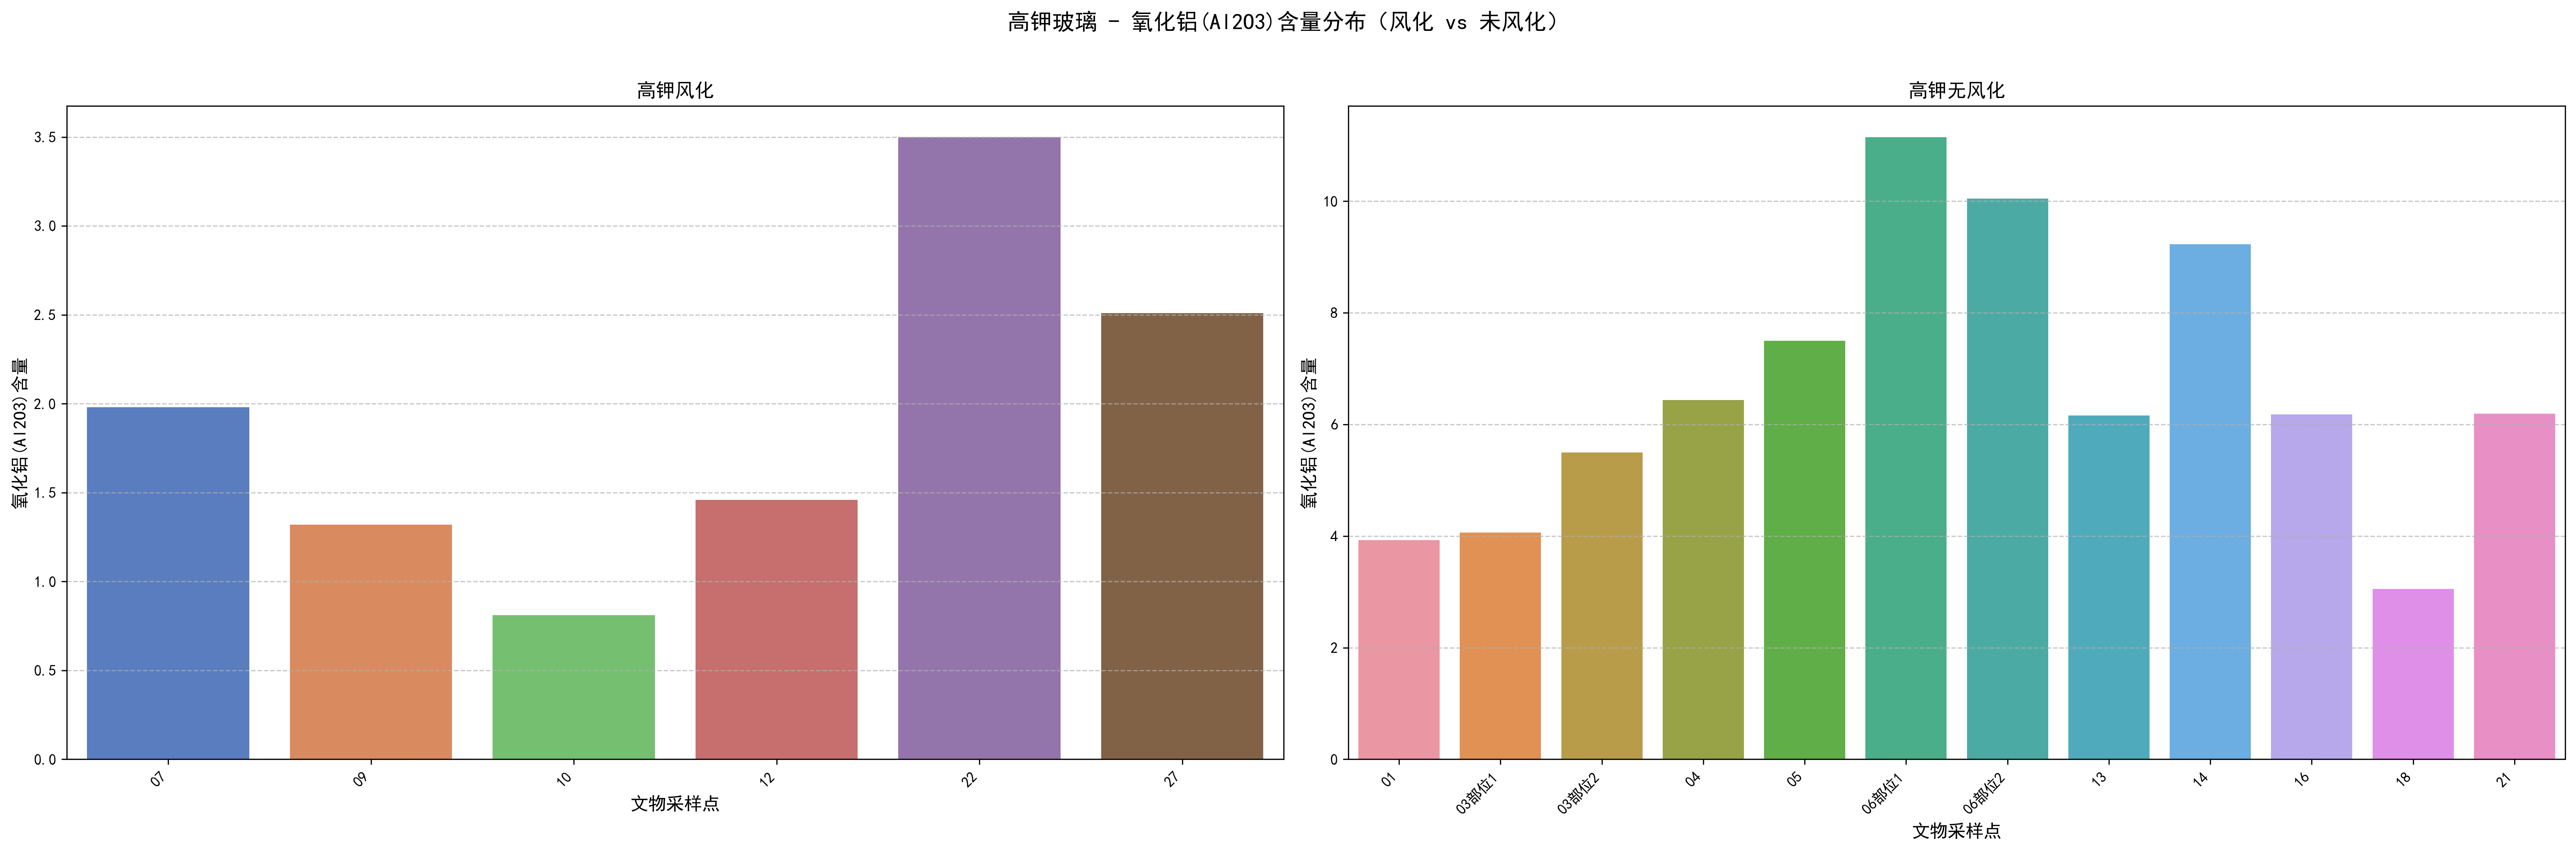
\includegraphics[width=0.9\textwidth]{figures/1.2/高钾玻璃 - 氧化铝(Al2O3)含量分布(风化 vs 未风化).png}
\caption{高钾玻璃 - 氧化铝(Al$_2$O$_3$)风化前后含量分布}
\label{fig:高钾玻璃 - 氧化铝(Al$_2$O$_3$)风化前后含量分布}
\end{figure}

\begin{figure}[H]
\centering
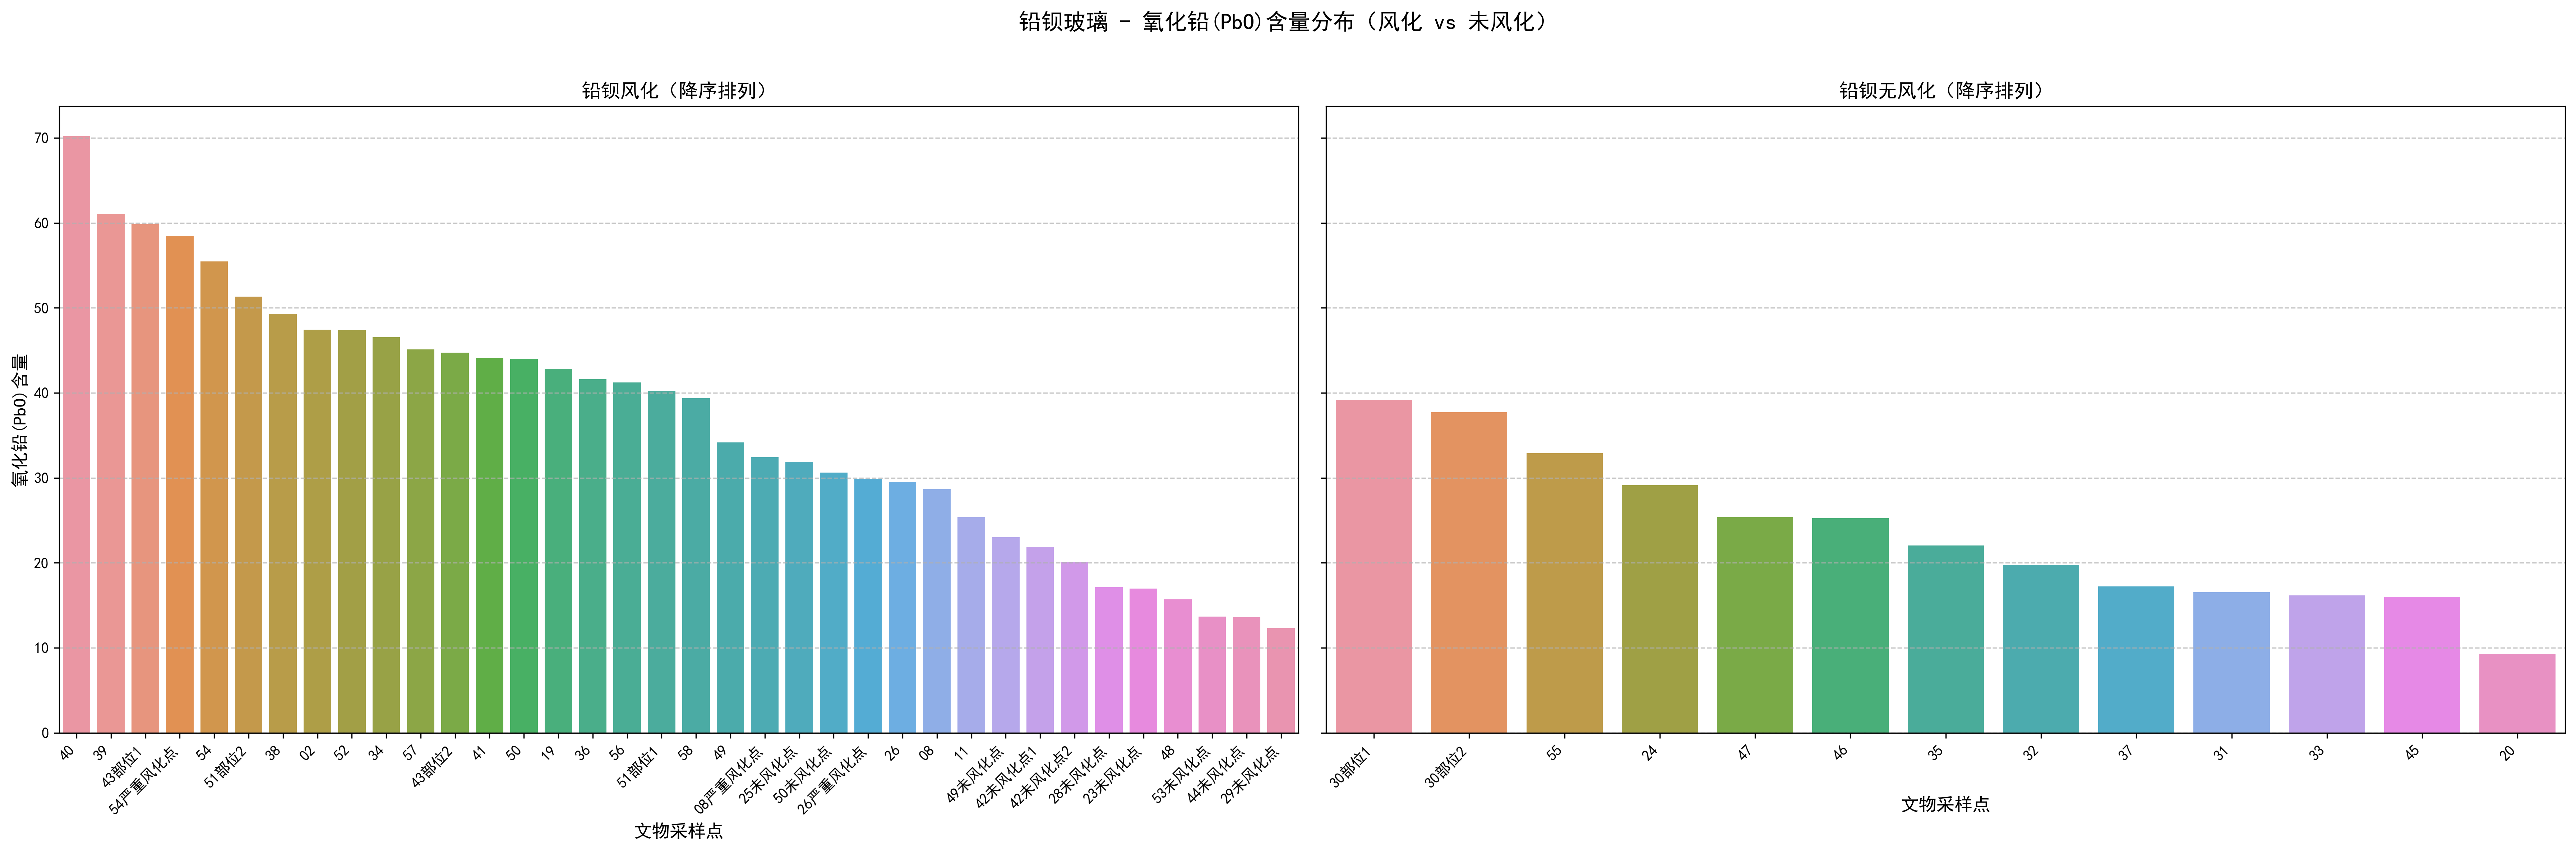
\includegraphics[width=0.9\textwidth]{figures/1.2/铅钡玻璃 - 氧化铅(PbO)含量分布(风化 vs 未风化).png}
\caption{铅钡玻璃 - 氧化铅(PbO)风化前后含量分布}
\label{fig:铅钡玻璃 - 氧化铅(PbO)风化前后含量分布}
\end{figure}

通过这些图表,可以直观地观察到:

\begin{itemize}
    \item 铅钡玻璃在风化后,SiO$_2$含量略微增加,而 SrO、Fe$_2$O$_3$、CuO、Na$_2$O、MgO、CaO、K$_2$O、Al$_2$O$_3$、PbO、BaO、P$_2$O$_5$ 和 SO$_2$ 含量均有不同程度的下降;
    \item 高钾玻璃在风化后,SiO$_2$含量显著降低,而 SrO、Fe$_2$O$_3$、CuO、Na$_2$O、MgO、CaO、K$_2$O、Al$_2$O$_3$、PbO、BaO、P$_2$O$_5$ 和 SO$_2$ 含量明显增加,SnO$_2$含量基本不变;
    \item 风化过程对不同类型玻璃的化学成分影响存在明显差异。
\end{itemize}

\subsection{风化前的化学成分含量的预测}

\subsubsection{数据分析}

通过阅读数据,我们发现,除了编号为49、50的样本具有成对的(风化前,风化后)的化学成分数据,
其他的样本都是基于风化前后两群体的横截面数据,可以抽象为(风化前,NULL)或(NULL,风化后)
的形式。同时,考虑到需要预测的是化学成分,是总和为1的成分数据,各成分之间彼此依赖,
不适宜使用一般的回归模型。

因此,我们基于成分数据分析CoDA模型,参考文献\cite{司守奎2011数学建模算法与应用},
在模型中添加先验正则项,最终建立风化前化学含量预测模型。

\subsubsection{模型记号与数据映射}

\begin{itemize}
\item 模型记号
\begin{itemize}
    \item $\mathbf{a}_i$ \quad (原始成分百分比)  
    \item $\mathbf{p}_i$ \quad (闭合后,和为 1 的比例)  
    \item $\mathbf{z}_i$ \quad (clr 后的向量)  
    \item $\bar{\mathbf{z}}_\text{w},\, \bar{\mathbf{z}}_\text{u}$ \quad  
    \item $\boldsymbol{\delta}_0$ \quad (按玻璃类型用文献导向值初始化)  
    \item $\mathbf{w}$ \quad (按成分设置权重)  
    \item $\lambda$ \quad (正则强度) 
    \item $n$ \quad (样本数)
\end{itemize}

\item 令成分列为:
\[
    \mathcal{P} = \{\mathrm{SiO}_2, \mathrm{Na}_2\mathrm{O}, \mathrm{K}_2\mathrm{O}, \ldots, \mathrm{SO}_2, \text{unknown}\}
\]
共 $D = 15$ 个成分

\item 将每行按百分比除以 100 进行闭合,得到组成比例矩阵 $\mathbf{p} \in \mathbb{R}^{n \times D}$。
    \begin{itemize}
        \item 样本 $i$ 的成分向量为 $\mathbf{a}_i$,闭合后
        \[
        \mathbf{p}_i = \mathcal{C}(\mathbf{a}_i) = \frac{\mathbf{a}_i}{\sum_{j=1}^D a_{ij}}, \quad \sum_{j=1}^D p_{ij} = 1.
        \]
    \end{itemize}

\item 为避免 $\log(0)$,在闭合前/或闭合后对零值做微小替换(伪计数)$\varepsilon$。

\item CLR 变换(把单纯形映到实向量空间):对每行 $i$
    \[
    \mathbf{z}_i = \text{clr}(\mathbf{p}_i) = \left( \ln \frac{p_{i1}}{g_i}, \ldots, \ln \frac{p_{iD}}{g_i} \right), \quad g_i = \left( \prod_{j=1}^D p_{ij} \right)^{1/D},
    \]
\end{itemize}

\subsubsection{风化模型}

我们在 CLR 空间做建模,主要假设(能使问题可解且可解释):

\textbf{线性位移假设}\quad 对同类玻璃,风化后与风化前在 CLR 空间上满足近似的平移关系(均值差):  
\[
\mathbf{z}_\text{w} \approx \mathbf{z}_\text{pre} + \boldsymbol{\delta} + \boldsymbol{\varepsilon},
\]  
其中 $\boldsymbol{\delta}$ 是同类玻璃的平均风化位移向量(在 CLR 空间),$\boldsymbol{\varepsilon}$ 是噪声。  

这样就可以得到基于群体差的回推策略而不需要成对样本。  

\begin{itemize}
\item 设 $\bar{\mathbf{z}}_\text{w}$、$\bar{\mathbf{z}}_\text{u}$ 分别为风化与未风化样本在 CLR 空间的均值,观测到的平均位移为:  
\[
\hat{\boldsymbol{\delta}}_\text{obs} = \bar{\mathbf{z}}_\text{w} - \bar{\mathbf{z}}_\text{u}.
\]  

\item 对任一风化样点 $i$,其风化前的 CLR 估计为:  
\[
\hat{\mathbf{z}}_\text{pre},_i^\text{(pure)} = \mathbf{z}_{\text{w},i} - \hat{\boldsymbol{\delta}}_\text{obs}.
\]  

\item 然后逆 CLR 得到比例并乘以 100 得到百分比:  
\[
\hat{\mathbf{p}}_{\text{pre},i} = \text{clr}^{-1}\!\left( \hat{\mathbf{z}}_{\text{pre},i} \right) 
= \frac{\exp\!\left( \hat{\mathbf{z}}_{\text{pre},i} \right)}{\sum_{k=1}^D \exp\!\left( \hat{z}_{\text{pre},i,k} \right)}.
\]  
\end{itemize}

\subsubsection{将文献先验融合进CoDA模型}

为了把“机理知识”引入(例如高钾玻璃倾向于 $\mathrm{K}_2\mathrm{O}$ 严重流失、
$\mathrm{SiO}_2$ 相对富集;铅钡体系可能出现 $\mathrm{Pb}/\mathrm{Ba}$ 比例变化与硫酸盐富集等),
我们在 CLR 空间对 $\boldsymbol{\delta}$ 加带方向性的岭惩罚:

\begin{itemize}

\item 设观测到的 $\boldsymbol{d} = \hat{\boldsymbol{\delta}}_{\text{obs}}$。我们引入先验中心向量 $\boldsymbol{\delta}_0$(来源于机理/文献方向性),以及对每个成分的权重向量 $\mathbf{w} = (w_1, \ldots, w_D)$(表示你对该分量先验的信心和强度),并设正则强度为 $\lambda \geq 0$。最小化目标:
\[
\min_{\boldsymbol{\delta}} \|\boldsymbol{\delta} - \boldsymbol{d}\|_2^2 + \lambda \|\mathbf{W}(\boldsymbol{\delta} - \boldsymbol{\delta}_0)\|_2^2,
\]
其中 $\mathbf{W} = \text{diag}(\mathbf{w})$。这是二次型问题,有闭式解:
\[
\hat{\boldsymbol{\delta}}_{\text{reg}} = (\mathbf{I} + \lambda \mathbf{W}^2)^{-1} (\boldsymbol{d} + \lambda \mathbf{W}^2 \boldsymbol{\delta}_0).
\]

当 $\lambda = 0$ 或者 $\mathbf{w} = 0$ 时,退化为纯数据驱动($\hat{\boldsymbol{\delta}} = \boldsymbol{d}$)。当 $\lambda$ 较大且某些 $w_j$ 很大时,$\hat{\boldsymbol{\delta}}$ 会更靠近 $\boldsymbol{\delta}_0$(先验主导)。

\end{itemize}

\subsubsection{先验权重$\lambda$和噪声$\epsilon$的调优}

基于已知文物编号49、50风化前后的化学成分变化,我们将其作为测试集,通过网格搜索来寻找
先验权重$\lambda$和噪声$\epsilon$的最优值。我们使用以下公式检验模型性能:

\[
	\text{MAE}_{\text{prior\_percent}} = \frac{\text{MAE}_{\text{model}}}{\text{MAE}_{\text{prior}}} \times 100\%
\]
\[
	\text{其中}\quad
	\text{MAE}_{\text{model}} = \frac{1}{n} \sum_{i=1}^{n} \left| y_i - \hat{y}_i \right|, \quad
	\text{MAE}_{\text{prior}} = \frac{1}{n} \sum_{i=1}^{n} \left| y_i - p_i \right|
\]

经过网格搜索,最终得到化学成分预测模型如下:

% ---------- 主公式 + 子公式 + 约束 ----------
\begin{align}
\widehat{\mathbf{a}}_{i,\mathrm{pre}}^{\mathrm{prior}} (\%)
&= 100 \cdot 
\frac{\exp\!\left( \mathbf{z}_i - \widehat{\boldsymbol\delta}_g^{\mathrm{prior}} \right)}
{\mathbf{1}^\top \exp\!\left( \mathbf{z}_i - \widehat{\boldsymbol\delta}_g^{\mathrm{prior}} \right)},
\\
\text{其中} \quad
\widehat{\boldsymbol\delta}_g^{\mathrm{prior}}
&= \left( \mathbf{I} + \lambda \mathbf{W}_g^2 \right)^{-1} 
\left[ \mathbf{d}_g + \lambda \mathbf{W}_g^2 \, \boldsymbol{\delta}_{0,g} \right],
\\
\text{s.t.} \quad &
\begin{cases}
\lambda \ge 0, \quad \mathbf{w}_g \in \mathbb{R}_{\ge 0}^D, \\[0.3em]
\boldsymbol{\delta}_{0,g} \in \mathcal{H}, \quad \mathbf{d}_g \in \mathcal{H}, \quad \mathbf{z}_i \in \mathcal{H}, \\[0.3em]
\mathcal{H} = \left\{ \mathbf{z} \in \mathbb{R}^D \ \bigg| \ \sum_{j=1}^D z_j = 0 \right\}, \\[0.3em]
\mathbf{p} \in \mathcal{S}^D, \quad 
\mathcal{S}^D = \left\{ \mathbf{p} \in \mathbb{R}_{>0}^D \ \bigg| \ \sum_{j=1}^D p_j = 1 \right\}, \\[0.3em]
\mathbf{W}_g = \mathrm{diag}(w_{g1}, \dots, w_{gD}), \quad w_{gj} \ge 0, \ \forall j, \\[0.3em]
i \in S_g^{(w)} \ \Rightarrow \ g \ \text{是样本 $i$ 的玻璃类型标签}.
\end{cases}
\end{align}




\smallskip
\noindent
\textit{参考链接:} \url{legest.ufpr.br}, \url{econ-papers.upt.edu}

%引用\cref{fig:单图}。

\begin{figure}[ht]
\centering
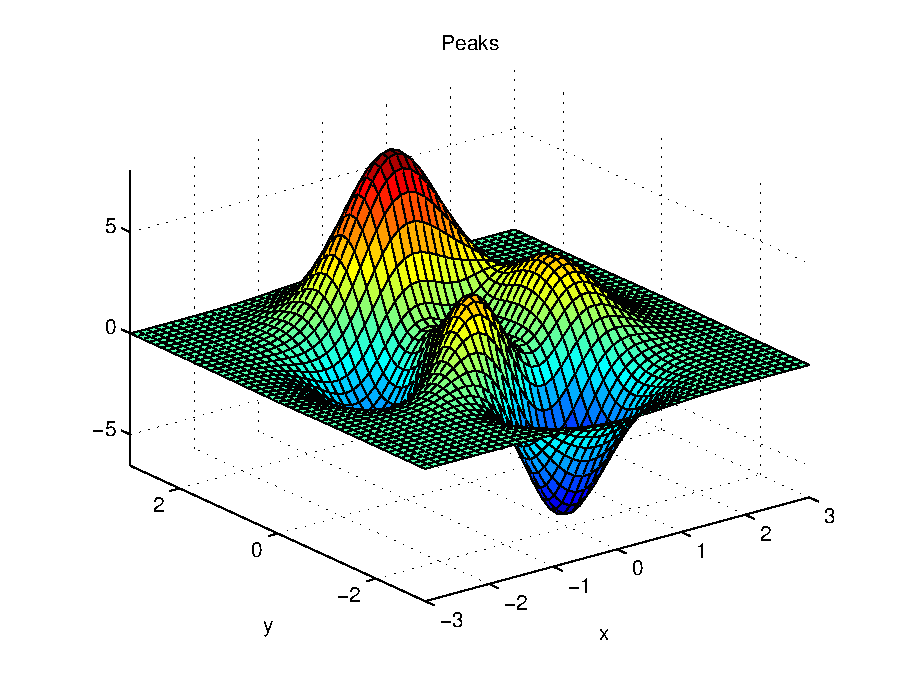
\includegraphics[width=0.75\textwidth]{example.eps}
\caption{单图}
\label{fig:单图}
\end{figure}

这句话引用了文献\cite{司守奎2011数学建模算法与应用}。

这句话引用了文献\upcite{卓金武2011MATLAB}。

\subsection{模型求解}

\textbf{Step1:} 

\textbf{Step2:} 

\textbf{Step3:} 

\subsection{求解结果}


%%%%%%%%%%%%%%%%%%%%%%%%%%%%%%%%%%%%%%%%%%%%%%%%%%%%%%%%%%%%% 

\section{问题二的模型的建立和求解}
\subsection{模型建立}

引用\cref{fig:双图},引用\cref{fig:双图a},引用\cref{fig:双图b}。

\begin{figure}[ht]
\centering
\subcaptionbox{双图a子标题\label{fig:双图a}}
{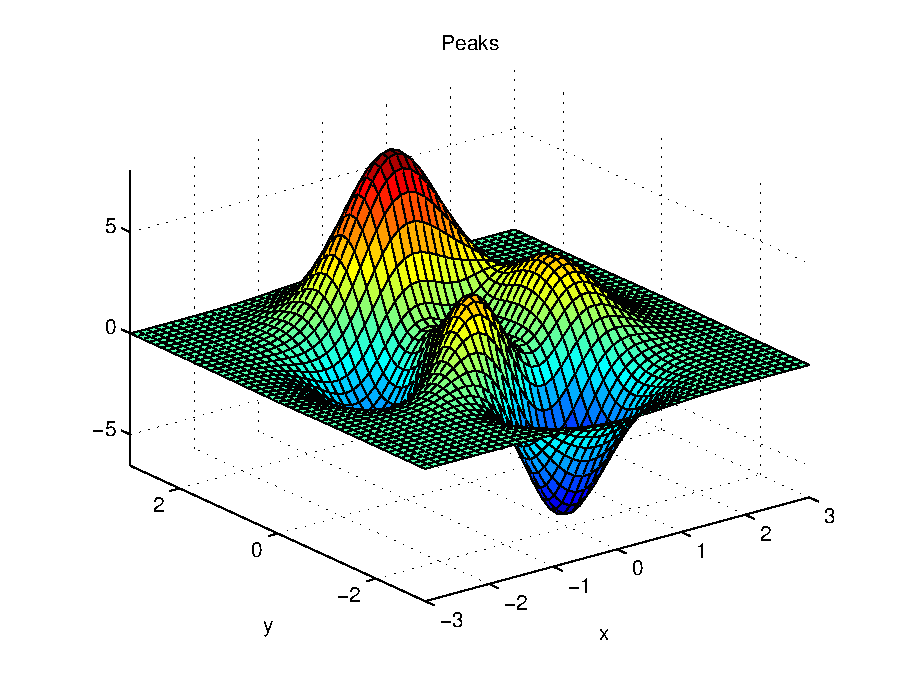
\includegraphics[width=.4\textwidth]{example.eps}}
\subcaptionbox{双图b子标题\label{fig:双图b}}
{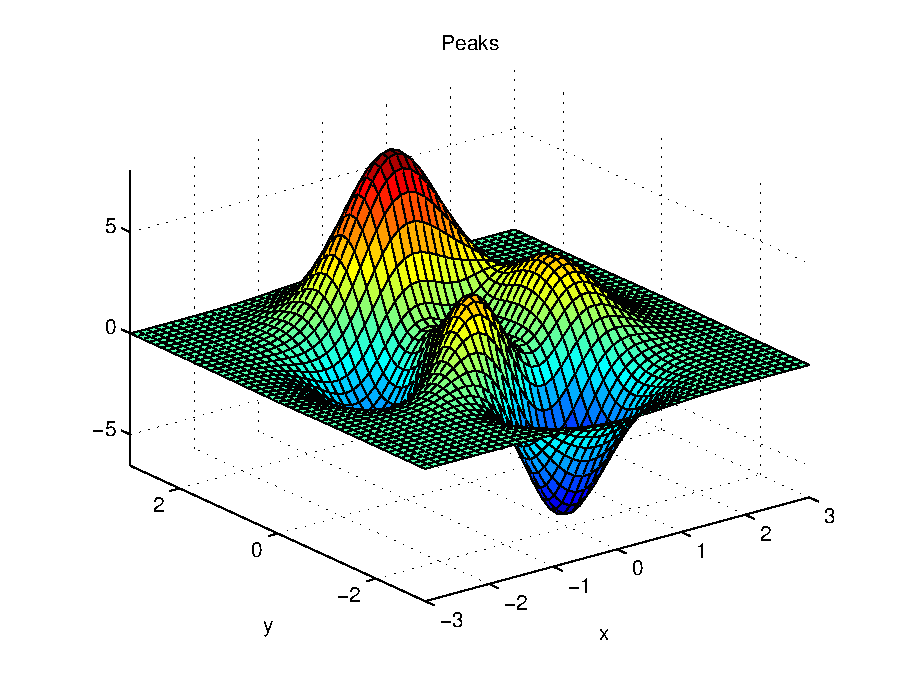
\includegraphics[width=.4\textwidth]{example.eps}}
\caption{双图}\label{fig:双图}
\end{figure} 

\subsection{模型求解}

\textbf{Step1:} 

\textbf{Step2:} 

\textbf{Step3:} 

\subsection{求解结果}

%%%%%%%%%%%%%%%%%%%%%%%%%%%%%%%%%%%%%%%%%%%%%%%%%%%%%%%%%%%%% 

\section{问题三的模型的建立和求解}
\subsection{模型建立}

\subsection{模型求解}

\textbf{Step1:} 

\textbf{Step2:} 

\textbf{Step3:} 

\subsection{求解结果}

%%%%%%%%%%%%%%%%%%%%%%%%%%%%%%%%%%%%%%%%%%%%%%%%%%%%%%%%%%%%% 

\section{问题四的模型的建立和求解}
\subsection{模型建立}

\subsection{模型求解}

\textbf{Step1:} 

\textbf{Step2:} 

\textbf{Step3:} 

\subsection{求解结果}

%%%%%%%%%%%%%%%%%%%%%%%%%%%%%%%%%%%%%%%%%%%%%%%%%%%%%%%%%%%%%

\section{模型的分析与检验}

\subsection{灵敏度分析}

\subsection{误差分析}

%%%%%%%%%%%%%%%%%%%%%%%%%%%%%%%%%%%%%%%%%%%%%%%%%%%%%%%%%%%%%

\section{模型的评价}

\subsection{模型的优点}
\begin{itemize}[itemindent=2em]
\item 优点1
\item 优点2
\item 优点3
\end{itemize}

\subsection{模型的缺点}
\begin{itemize}[itemindent=2em]
\item 缺点1
\item 缺点2
\end{itemize}

%%%%%%%%%%%%%%%%%%%%%%%%%%%%%%%%%%%%%%%%%%%%%%%%%%%%%%%%%%%%%
%% 参考文献
\nocite{*}
\bibliographystyle{gbt7714-numerical}  % 引用格式
\bibliography{ref.bib}  % bib源

\newpage
%%%%%%%%%%%%%%%%%%%%%%%%%%%%%%%%%%%%%%%%%%%%%%%%%%%%%%%%%%%%%
%% 附录
\begin{appendices}
\section{文件列表}
\begin{table}[H]
\centering
\begin{tabularx}{\textwidth}{LL}
\toprule
文件名   & 功能描述 \\
\midrule
q1.m & 问题一程序代码 \\
q2.py & 问题二程序代码 \\
q3.c & 问题三程序代码 \\
q4.cpp & 问题四程序代码 \\
\bottomrule
\end{tabularx}
\label{tab:文件列表}
\end{table}

\section{代码}
\noindent q1.m
\lstinputlisting[language=matlab]{code/q1.m}
q2.py
\lstinputlisting[language=python]{code/q2.py}
q3.c
\lstinputlisting[language=c]{code/q3.c}
q4.cpp
\lstinputlisting[language=c++]{code/q4.cpp}
\end{appendices}
\end{document}


%%%%%双图模板%%%%%%
\begin{figure}
\centering
\subcaptionbox{炉温曲线示意图\label{fig:双图a}}
{\includegraphics[width=.4\textwidth]{炉温曲线示意图.png}}
\subcaptionbox{问题1炉温曲线\label{fig:双图b}}
{\includegraphics[width=.4\textwidth]{问题1炉温曲线.png}}
\caption{双图}\label{fig:双图}
\end{figure} 
%%%%%双图模板%%%%%%